\section{前言}

隨著智慧型機器人與人工智慧的蓬勃發展,近年來各國均投入於無人載具之開發與研究,已經在非常多場域漸漸出現。在有結構性的環境(structured environments)下,無人駕駛車在從室外之高速公路、郊外人車較少之公路,到室內工廠物流運輸機器人系統已經有相當成熟的發展,其原因在於其所產生的應用是非常貼切人類的日常生活,並且能創造更大之經濟效應,例如:交通工具、商業物流等。但在意外發時,例如:輻射外洩。等人類無法進入之嚴峻場地,機器人更能發揮其不可取代性,代替人類進入災區進行移動、導航、定位、救援。

\begin{figure}[t]
  \centering
    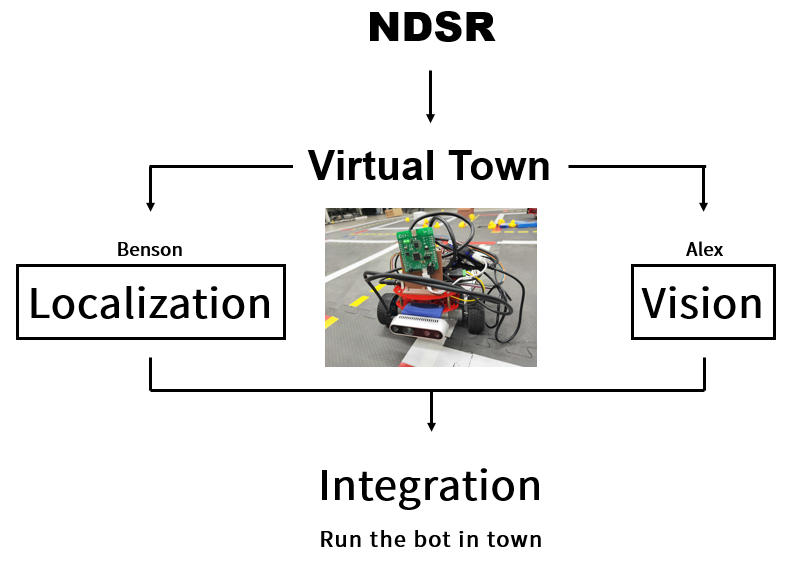
\includegraphics[width=\columnwidth]{images/teaser.png}
        \caption{本計畫目標為建置整合機器人搜救系統,包括UWB定位及MobileNet-SSD目標偵測,能夠清楚知道目標搜救物位於地圖中的何處,於Duckietown場地進行驗證。}
 \label{figure:teaser}
\end{figure}

國防科技一直以來是各個國家的發展重點。美國國防高等研究計劃署 (Defense Advanced Research Projects Agency, DARPA)以及美國太空總署(NASA)針對這樣的挑戰, 舉辦相關競賽,如:DARPA Subterranean Challenge(簡稱SubT),這場競賽旨在開發能夠「探索快速繪製、導航、搜索和開發複雜地下環境的新方法」,包括人造隧道系統、城市地下和自然洞穴網絡等。大賽要求參賽者研製出能幫助人類在地下導航、繪圖以及搜尋的系統,所有救援系統在地下結構發生塌方或其他災難時,能夠在對人類來說有危險的地方移動和導航,幫助救援。

而本次專題就是根據核災發生現場,或任何人員無法進入之場地、城市,由應變機器人進入災區偵測目標物,並且能夠在無GPS之場域進行定位,準確得知無人車輛目前位置與目標物之相對位置,讓搜救人員迅速進行偵查、救援。

\begin{figure*}[tb]
	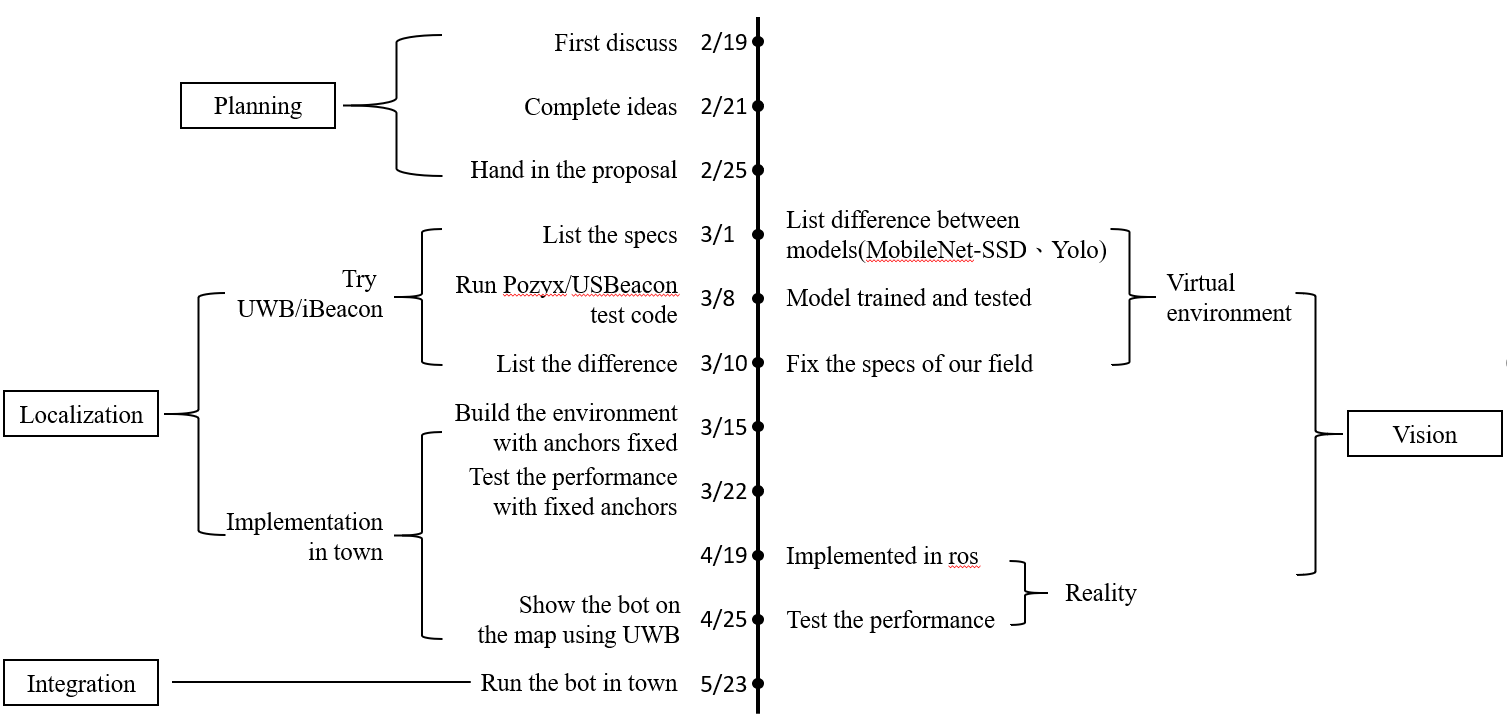
\includegraphics[width=1.8\columnwidth]{images/sys-architecture.png}
	\centering
	\caption{本專題之進度分工圖,博凱-Vision、聖誠-Localization}
	\label{figure:localization_sys_architecture}
\end{figure*}

綜合上述,此搜救機器人需具備立體視覺整合系統感知偵測目標物並與UWB定位結合,需考量目標物大小、定位準度、目標物深度資訊等等計算出相對位置,因此,本報告的目標與貢獻如下:

\begin{enumerate}
\item
UWB定位及MobileNet-SSD目標辨識
\item 
合併且整合系統
\item 
將結果可視化並顯示於Rviz
\end{enumerate}







